%\begin{frame}
%    \centering
%    \Large{Part II:}\\
%    \ \\
%    \ \\
%    \centering
%    \Large{Linear scaling Coulomb interaction in the multiwavelet basis,\\
%	a parallel implementation}
%\end{frame}

%\begin{frame}
%    \frametitle{Operator representation}
%    \begin{columns}
%    \begin{column}[b]{0.5\linewidth}
%    \begin{itemize}
%	\item	The multiwavelet basis is well suited for\\ 
%        \textbf{integral convolution operators}
%	    \begin{equation}
%		\nonumber
%		g(\boldsymbol{r}) = \left[T f\right](\boldsymbol{r}) = 
%		    \int K(\boldsymbol{r} - \boldsymbol{r'})f(\boldsymbol{r'}) d\boldsymbol{r'}
%	    \end{equation}
%	    \ \\
%	    \ \\
%	\item \textbf{Scaling projection} of operator at scale $n$
%	    \begin{equation}
%		\nonumber
%		T \approx T^n
%	    \end{equation}
%	\item \textbf{Wavelet projections} obtained by the difference
%	    \begin{equation}
%		\nonumber
%		T^{n+1} - T^n = A^n + B^n + C^n
%	    \end{equation}
%	\item \textbf{Multiresolution operator} obtained by recursion
%	    \begin{equation}
%		\nonumber
%		T^N = T^0 + \sum_{n=0}^{N-1} \left[A^n + B^n + C^n\right]
%	    \end{equation}
%	\item Scaling operator $T$ is \textbf{dense}
%	\item Wavelet operators $A$, $B$ and $C$ are \textbf{sparse} 
%    \end{itemize}
%    \end{column}
%    \begin{column}[b]{0.5\linewidth}
%    \begin{center}
%    \only<2>{\hspace{4.0mm}
%    \includegraphics[scale=0.6, clip, viewport = 240 280 450 480]
%    {figures/matrix/matrix_1.pdf}
%    }
%    \only<3>{\hspace{3.4mm}
%    \includegraphics[scale=0.6, clip, viewport = 240 280 450 480]
%    {figures/matrix/matrix_2.pdf}
%    }
%    \only<4>{\hspace{2.8mm}
%    \includegraphics[scale=0.6, clip, viewport = 240 280 450 480]
%    {figures/matrix/matrix_3.pdf}
%    }
%    \only<5>{\hspace{2.2mm}
%    \includegraphics[scale=0.6, clip, viewport = 240 280 450 480]
%    {figures/matrix/matrix_4.pdf}
%    }
%    \only<6>{\hspace{1.6mm}
%    \includegraphics[scale=0.6, clip, viewport = 240 280 450 480]
%    {figures/matrix/matrix_5.pdf}
%    }
%    \only<7>{\hspace{1mm}
%    \includegraphics[scale=0.6, clip, viewport = 240 280 450 480]
%    {figures/matrix/matrix_6.pdf}
%    }
%    \vspace{5mm}
%    \end{center}
%    \end{column}
%    \end{columns}
%    \vspace{5mm}
%
%    \begin{columns}
%    \begin{column}{.48\textwidth}
%    \centering
%    \textbf{Poisson kernel}
%    \begin{equation}
%	\nonumber
%	P(\boldsymbol{r}-\boldsymbol{r}') = 
%	    \frac{1}{4\pi}\ \frac{1}{|\boldsymbol{r}-\boldsymbol{r}'|}
%    \end{equation}
%    \end{column}
%    \begin{column}{.48\textwidth}
%    \centering
%    \textbf{Helmholtz kernel}
%    \begin{equation}
%	\nonumber
%	H^{\mu}(\boldsymbol{r}-\boldsymbol{r}') = \frac{1}{4\pi}\ 
%	\frac{e^{-\mu |\boldsymbol{r}-\boldsymbol{r}'|}}
%        {|\boldsymbol{r}-\boldsymbol{r}'|}
%    \end{equation}
%    \end{column}
%    \end{columns}    
%    \centering
%    \vspace{8mm}
%    \tiny
%    G. Beylkin, R. Coifman, V. Rokhlin, 
%    {\it Commun. Pure Appl. Math.}
%    \textbf{44(2)}
%    (1991)
%\end{frame}

%\begin{frame}
%    \frametitle{Coulomb interaction}
%    \begin{itemize}
%	\item	Electrostatic potential from a \textbf{point charge} follows from Coulomb's law
%		\begin{equation}
%		    \nonumber
%		    V(\boldsymbol{r}) = \frac{q}{4\pi\epsilon_0}
%		    \frac{1}{|\boldsymbol{r}-\boldsymbol{r}'|}
%		\end{equation}
%		\ \\
%		\ \\
%		\ \\
%	\item	Electrostatic potential from a \textbf{charge density} is given by the Poisson equation
%		\begin{equation}
%		    \nonumber
%		    \nabla^2 V(\boldsymbol{r}) = -\rho(\boldsymbol{r})
%		\end{equation}
%		\ \\
%		\ \\
%		\ \\
%	\item	Can be solved directly in integral form using the Poisson kernel
%		\begin{equation}
%		    \nonumber
%		    V(\boldsymbol{r}) = 
%		    \int P(\boldsymbol{r}-\boldsymbol{r'})\rho(\boldsymbol{r'}) d\boldsymbol{r'} =
%		    \int\frac{\rho(\boldsymbol{r'})}{4\pi|\boldsymbol{r} - \boldsymbol{r'}|} d\boldsymbol{r'} 
%		\end{equation}
%		\ \\
%		\ \\
%		\ \\
%    \end{itemize}
%    \ \\
%    \ \\
%    \ \\
%    \begin{columns}
%    \begin{column}{.30\textwidth}
%        \ \\
%    \end{column}
%    \begin{column}{.40\textwidth}
%        \ \ \ \ \textbf{Numerical problems}
%        \begin{itemize}
%	    \item Not Cartesian separable
%	    \item Singularity at short-range
%	    \item Slow decay at long-range
%	\end{itemize}
%    \end{column}
%    \begin{column}{.30\textwidth}
%	\ \\
%    \end{column}
%    \end{columns}
%\end{frame}

%\begin{frame}
%    \frametitle{Separation of variables using Gaussians}
%    \centering
%    The Poisson equation is solved in integral form using the Poisson kernel
%    \begin{equation}
%	\nonumber
%	V(\boldsymbol{r}) = \int P(\boldsymbol{r}-\boldsymbol{r'})
%        \rho(\boldsymbol{r'}) d\boldsymbol{r'} =
%	\int\frac{\rho(\boldsymbol{r'})}
%        {4\pi|\boldsymbol{r} - \boldsymbol{r'}|} d\boldsymbol{r'} 
%    \end{equation}
%
%    \vspace{3mm}
%
%    \begin{columns}
%    \begin{column}{.50\textwidth}
%    \begin{itemize}
%	\item The Poisson kernel can be approximated as
%	    \begin{equation}
%		\nonumber
%		\frac{1}{\boldsymbol{r}} \approx 
%                \sum_{i=1}^M a_i e^{-\alpha_i \boldsymbol{r}^2} 
%	    \end{equation}
%	\item Any accuracy can in principle be obtained
%	\item Full operator is decomposed into $M$ terms
%	\item Each operator term is applied separately
%    \end{itemize}
%
%    \vspace{6mm}
%
%    \hspace{3mm} \textbf{Solves numerical problems}
%
%    \begin{itemize}
%	\item	Separates coordinates
%	\item	Removes singularity
%	\item	Separates length scales
%    \end{itemize}
%
%    \end{column}
%    \begin{column}{.50\textwidth}
%	\only<1>{\hspace{2mm}
%        \includegraphics[scale=0.4, clip, viewport = 110 450 490 800]
%            {figures/kernel_1.pdf}}
%	\only<2>{\hspace{2mm}
%        \includegraphics[scale=0.4, clip, viewport = 110 450 490 800]
%            {figures/kernel_2.pdf}}
%	\only<3>{\hspace{2mm}
%        \includegraphics[scale=0.4, clip, viewport = 110 450 490 800]
%            {figures/kernel_3.pdf}}
%	\only<4>{\hspace{2mm}
%        \includegraphics[scale=0.4, clip, viewport = 110 450 490 800]
%            {figures/kernel_4.pdf}}
%	\only<5>{\hspace{2mm}
%        \includegraphics[scale=0.4, clip, viewport = 110 450 490 800]
%            {figures/kernel_5.pdf}}
%	\only<6>{\hspace{2mm}
%        \includegraphics[scale=0.4, clip, viewport = 110 450 490 800]
%            {figures/kernel_6.pdf}}
%	\only<7>{\hspace{2mm}
%        \includegraphics[scale=0.4, clip, viewport = 110 450 490 800]
%            {figures/kernel_7.pdf}}
%	\only<8>{\hspace{0mm}
%        \includegraphics[scale=0.4, clip, viewport = 110 450 490 800]
%            {figures/kernel_7.pdf}}
%    \end{column}
%    \end{columns}    
%
%    \vspace{5mm}
%
%    \centering
%    \only<7>{\vspace{2mm}}
%    \only<1,2,3,4,5,6,7>{\vspace{6mm}
%    \tiny
%    G. Beylkin, M.J. Mohlenkamp,
%    {\it Proc. Nat. Acad. Sci.}
%    \textbf{99(16)}
%    (2002)
%    }
%    \only<8>{
%    \vspace{3mm}
%    \normalsize{Combined with the sparse wavelet representation of 
%    operators we get\\ \textbf{linear scaling algorithms}}
%    }
%\end{frame}

\begin{frame}
    \frametitle{Vanishing moments}
    \centering
    \textbf{A function $f$ has $M$ vanishing moments if}
    \begin{equation}
        \nonumber
        \mu_m = \int_0^1 x^m f(x) dx = 0,\qquad m = 0, 1, \dots, M - 1
    \end{equation}
    \ \\
    \ \\
    \ \\
    \begin{columns}
    \begin{column}{.15\textwidth}
        \ \\
    \end{column}
    \begin{column}{.85\textwidth}
    \begin{itemize}
        \item   Scaling basis has no vanishing moments $\longrightarrow$ 
		\textbf{long ranged} interaction
        \item   Wavelet basis has $k$ vanishing moments $\longrightarrow$ 
		\textbf{short ranged} interaction
    \end{itemize}
    \end{column}
    \end{columns}
    \ \\
    \ \\
    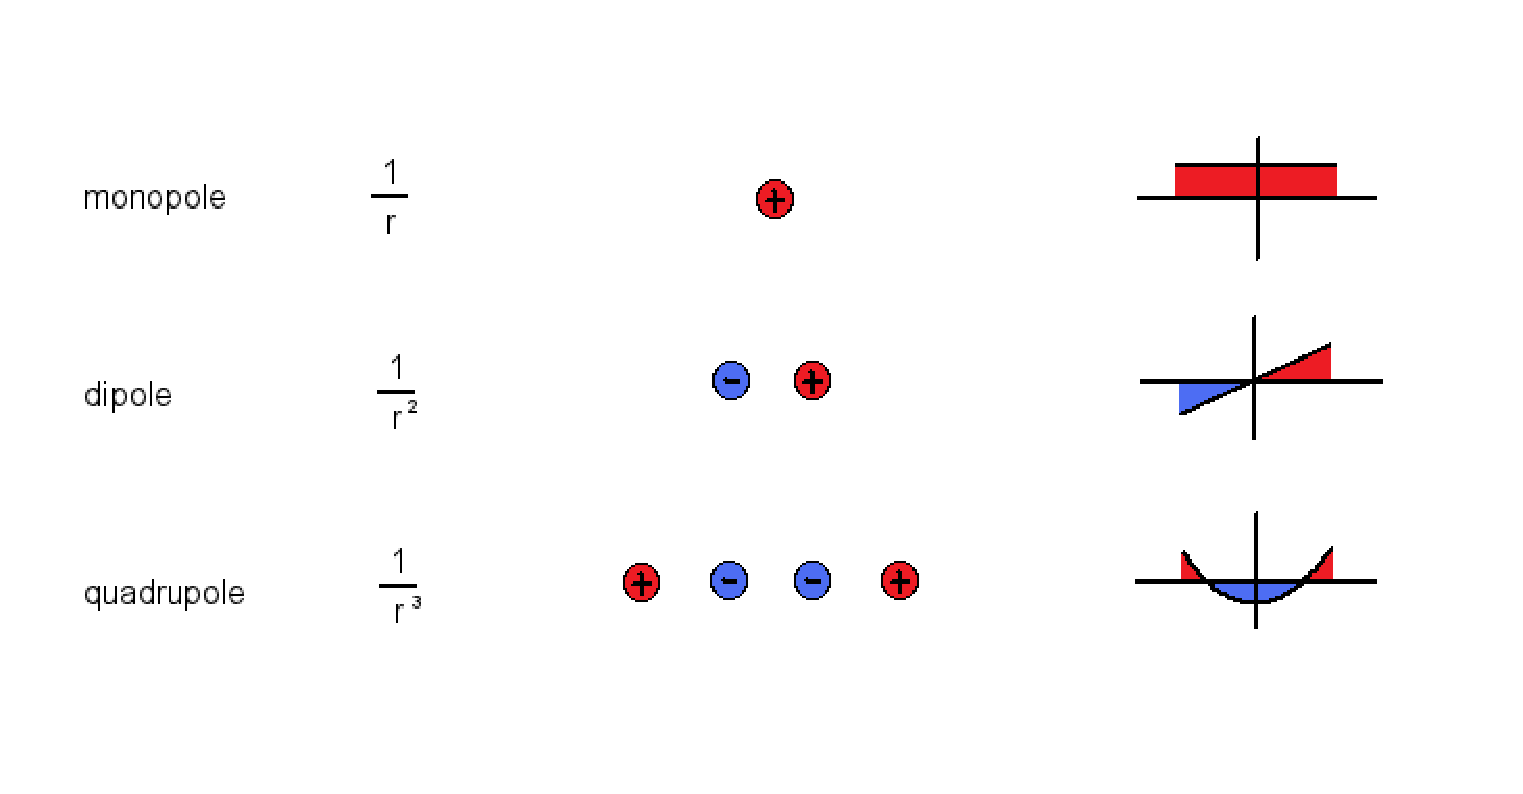
\includegraphics[scale=0.4, clip, viewport = 0 50 680 350]{figures/multipoles.pdf}
\end{frame}

%\begin{frame}
%    \frametitle{Algorithm}
%    \begin{algorithmic}[1]
%        \STATE create \tree skeleton of empty \nodes for the output function
%        \STATE create list of \emph{all} output \nodes
%        \WHILE{number of output \nodes in the current list $N>0$}
%            \FOR{each output \node in the current list}
%                \STATE fetch \emph{all} input \nodes within bandwidth of the \emph{full} operator
%                \STATE compute scaling and wavelet coefficients of output \node
%            \ENDFOR
%            \FOR{each \node of the output function}
%                \STATE remove \node from current list
%                \IF{\node needs to be refined}
%                    \STATE allocate children \nodes
%                    \STATE add children \nodes to the current list
%                \ENDIF
%            \ENDFOR
%        \ENDWHILE
%    \end{algorithmic}
%    \ \\
%    \ \\
%    \ \\
%    \pause
%    \begin{algorithmic}[1]
%        \FOR{each separated component ($\kappa = 1,\dots,M$) of the operator}
%            \FOR{each s/w component of output function}
%                \FOR{each s/w component of input function}
%                    \STATE fetch appropriate operator component (e.g. $T\times A\times A$)
%                    \STATE construct bandwidth
%                    \STATE fetch input and operator \nodes within bandwidth
%                    \STATE prune list of input \nodes based on Cauchy-Schwartz screening
%                    \FOR{each contributing input \node}
%                        \STATE apply operator
%                    \ENDFOR
%                \ENDFOR
%            \ENDFOR
%        \ENDFOR         
%    \end{algorithmic}
%\end{frame}


\begin{frame}
    \frametitle{Linear scaling Coulomb interaction}
    \begin{columns}
    \begin{column}{.10\textwidth}
    \ \\
    \end{column}
    \begin{column}{.40\textwidth}
	\centering
	\ \\
	\ \\
	\ \\
	\ \\
	\textbf{Alkane chains}
	\begin{equation}
	    \nonumber
	    C_{n}H_{2n+2}, \qquad n=2,\dots,70
	\end{equation}
	\ \\
	\ \\
	\ \\
	\textbf{Fitted curve}
	\begin{equation}
	    \nonumber
	    t(n) = 12.5 + 2.34n^{0.754} 
	\end{equation}
    \end{column}
    \begin{column}{.50\textwidth}
	\centering
	\begin{figure}
	    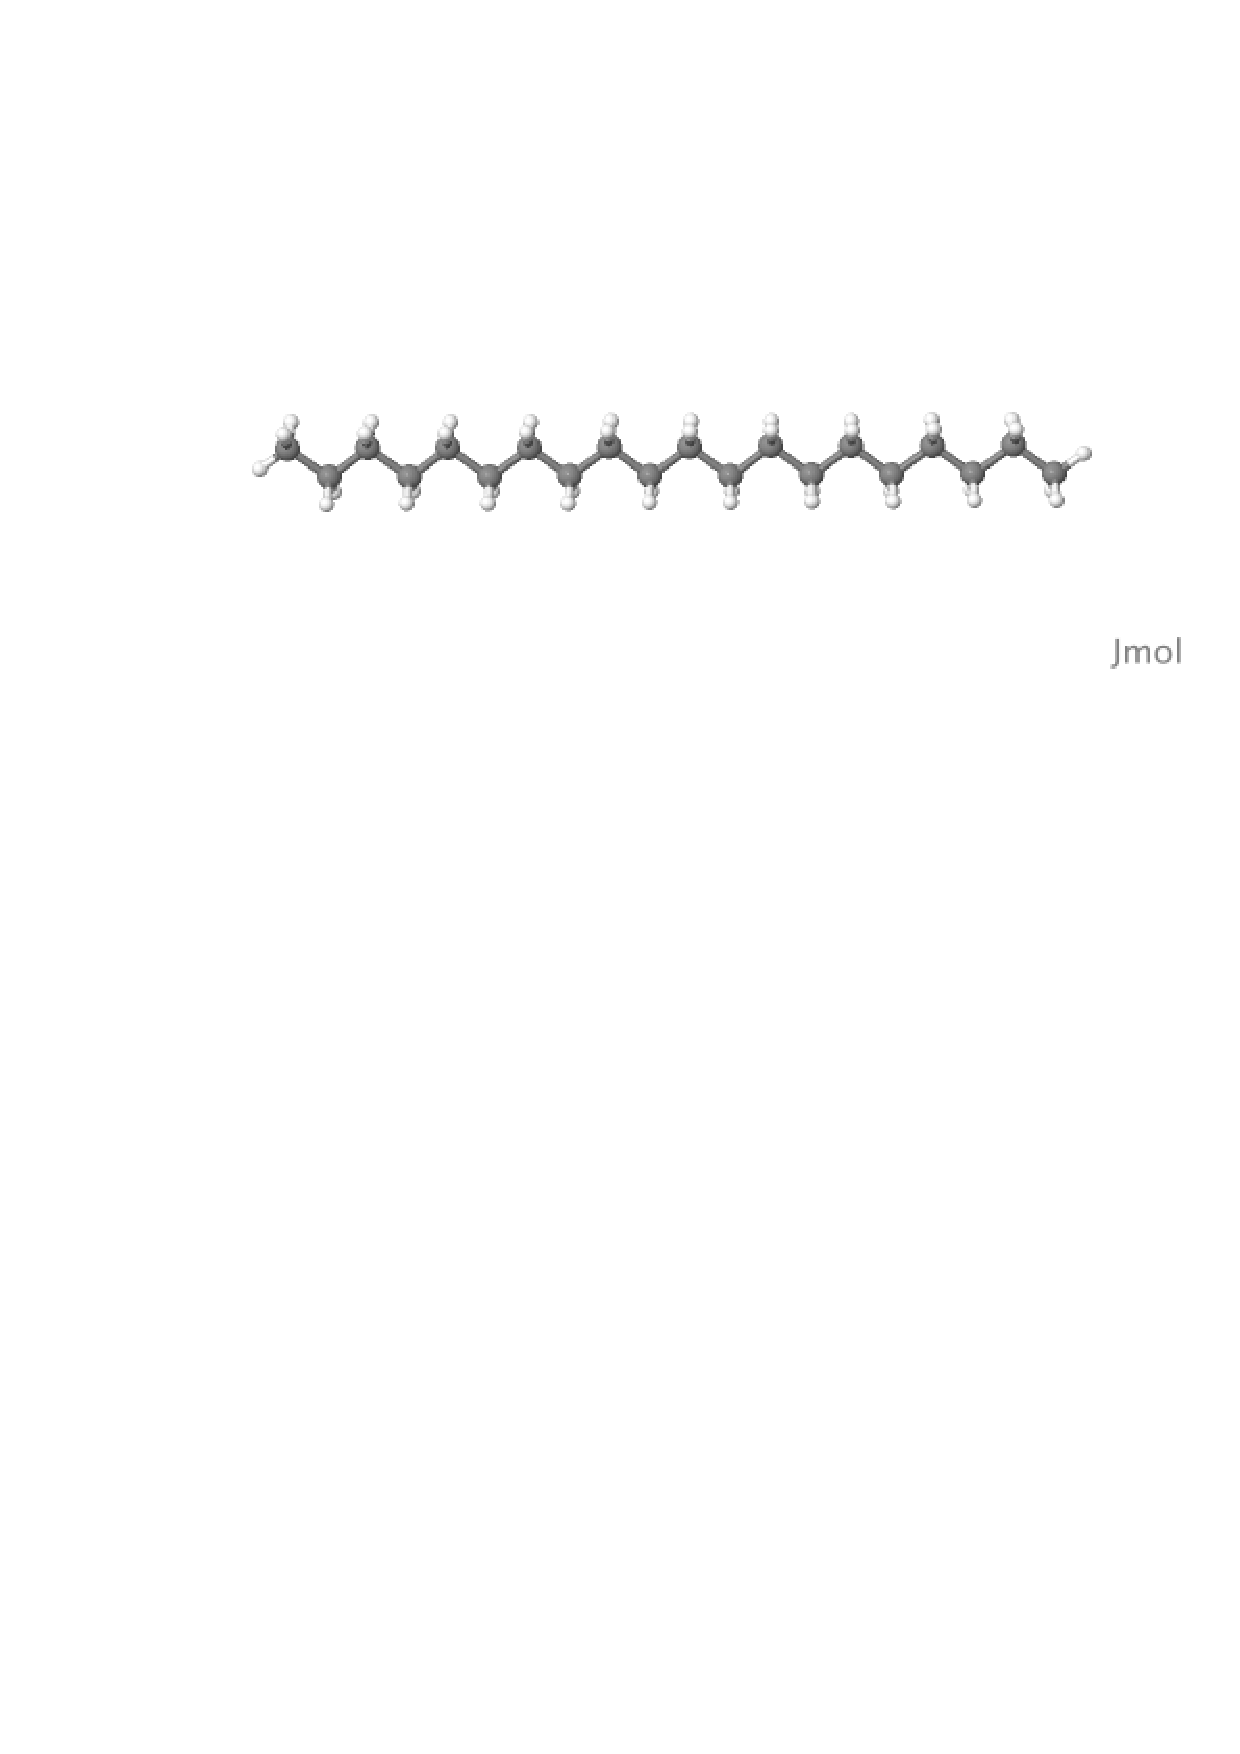
\includegraphics[scale=0.3, clip, viewport = 80 560 600 720]{figures/alkane.pdf}
	\end{figure}
	\textbf{Fitted curve}
	\begin{equation}
	    \nonumber
	    t(n) = -6.0 + 1.33n^{0.991}
	\end{equation}
	\ \\
	\ \\
    \end{column}
    \end{columns}    
    \ \\
    \begin{center}
	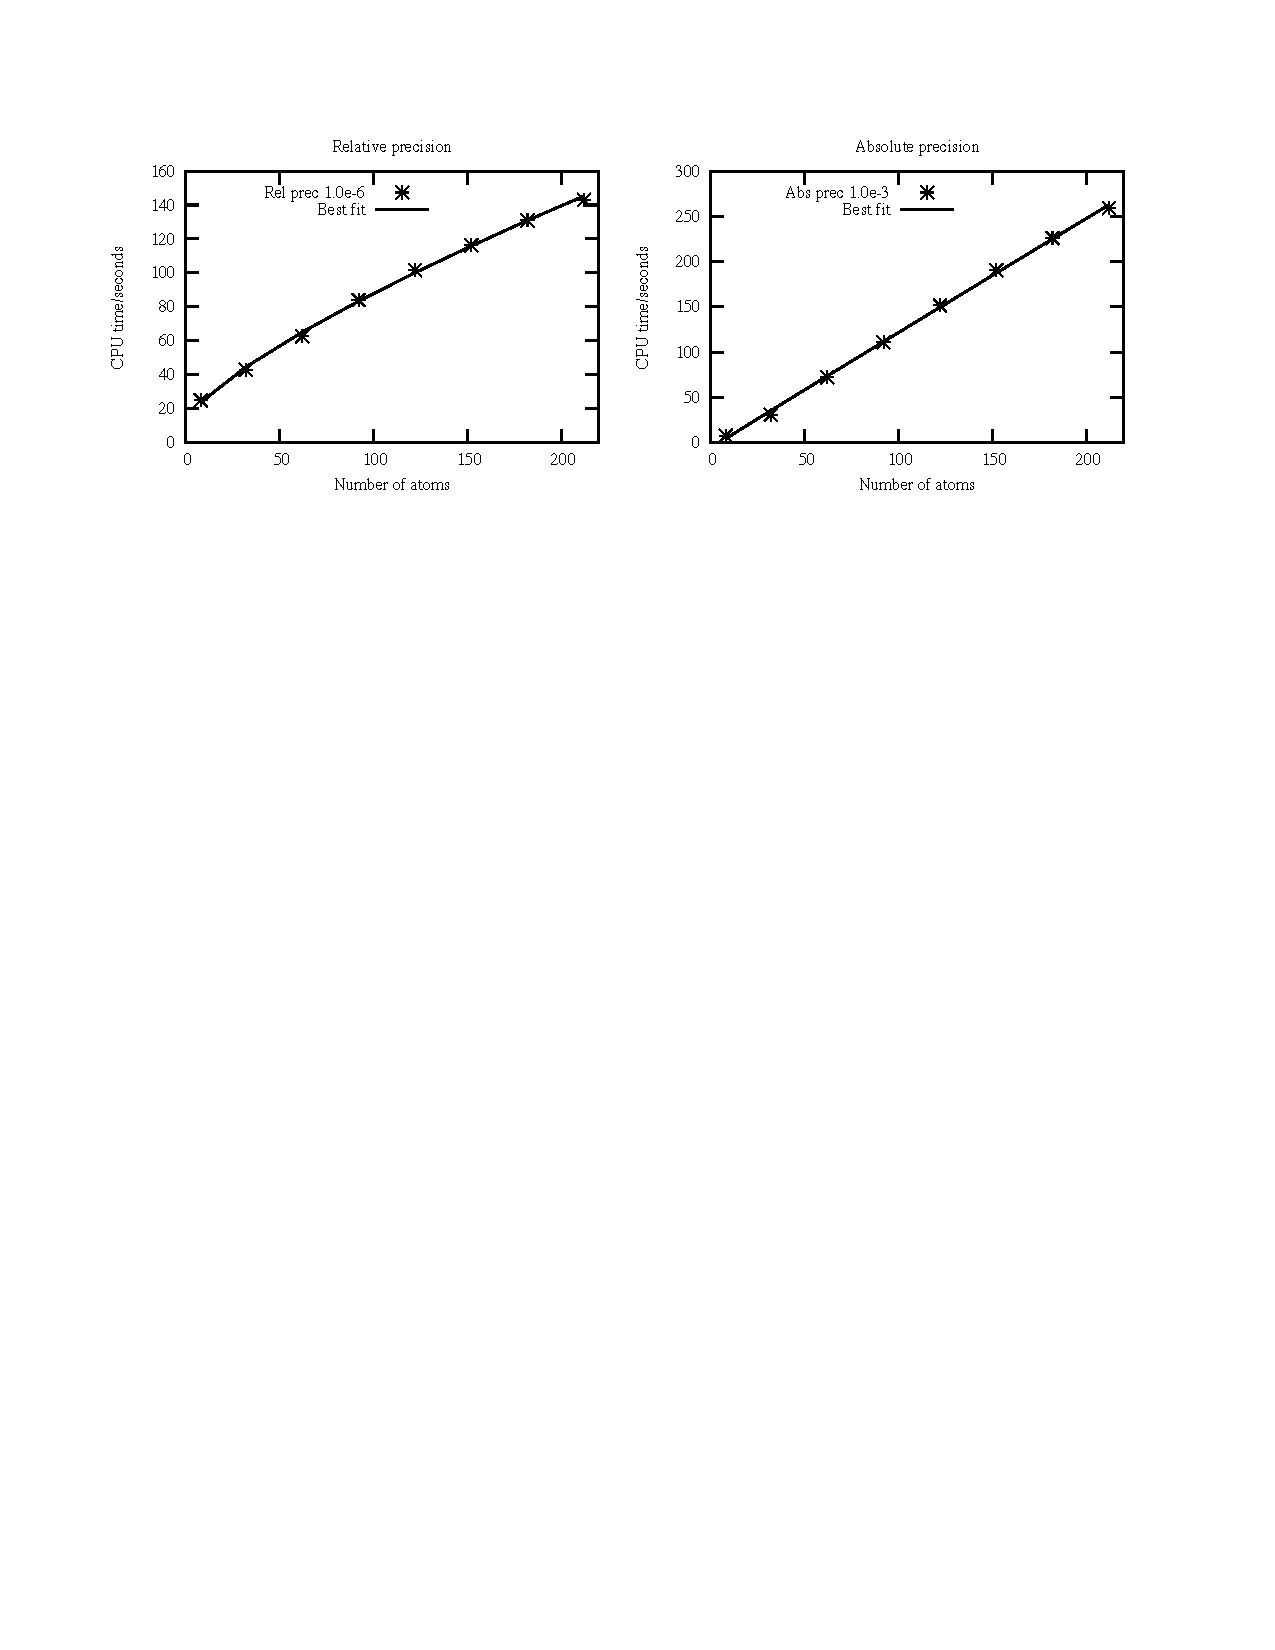
\includegraphics[scale=0.6, clip, viewport = 50 550 540 730]{figures/linearScaling.pdf}
    \end{center}

    \vspace{10mm}

\end{frame}


